\chapter{Lesson 3}
\section{Overview}
This third lesson will include both review material, and new material. We'll learn the three remaining open chords that are generally considered the basic chords. We'll also learn another strumming pattern, and an A Blues Scale. And, as with the previous lessons, we'll finish up by learning a few new songs that use these new techniques we've learned.

Are you ready? Good, let's begin lesson three.

\section{The Blues Scale}
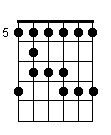
\includegraphics{partthree/bluesscale.png}

Before we jump into playing this useful new scale, let's review the fingers we will use to play the scale's notes. This scale is referred to as a "movable scale", meaning that we can play the scale anywhere on the neck. For now, we will play the scale starting on the fifth fret, but feel free to play it at the tenth fret, at the first fret, or anywhere else.

As with previous exercises, the blues scale requires precise fingering in your fretting hand in order for it to be most useful. All notes on the fifth fret will be played by the first finger. Notes on the sixth fret will be played by the second finger. Notes on the seventh fret will be played by the third finger. And all notes on the eighth fret will be played by the fourth finger.

One of the best ways to start working on the coordination in your fingers is to practice playing scales. Although they may seem boring, they will help build the strength and agility your fingers need to play the guitar well. Keep that in mind while practicing this new scale.

Count up to the fifth fret of your guitar. On most guitars, the fifth fret will be marked with a dot on the fretboard. Place your first finger on the fifth fret of the sixth string and play that note. Next, put your fourth (pinky) finger on the eighth fret of the sixth string, and again play that note. Now, continue to the fifth string, and follow the pattern illustrated above, until you've reached the eighth fret on the first string (listen to scale. Take your time and learn this scale well... it'll be one that you use often.

\subsection{Remember:}
\begin{itemize}
\item Use alternate picking.
\item Once you've finished the scale, try playing the scale backwards. Start at the first string, third fret, and play all notes in exactly the reverse order.
\item The key here is accuracy, not speed! Try playing the scale very slowly, making sure that each note is ringing clearly.
\end{itemize}

\section{Learning an E Major Chord}
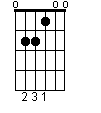
\includegraphics{partthree/openemajor.png}

Just a few more chords this week to fill in the ones we didn't cover previously. Once you've learned these three new chords, you'll know all of what are generally considered to be the basic open chords.

\subsection{Playing an E major chord}

Playing an Emajor chord is actually very similar to playing an Aminor chord; you just need to switch the strings you are playing the chord on. Start by placing your second finger on the second fret of the fifth string. Now, place your third finger on the second fret of the fourth string. Lastly, place your first finger on the first fret of the third string. Strum all six strings and you're playing an Emajor chord.

Now, like last lesson, test yourself to make sure you're playing the chord properly. Starting on the sixth string, strike each string one at a time, making sure each note in the chord is ringing clearly. If not, study your fingers, and identify what the problem is. Then, try to adjust your fingering so the problem goes away.

\section{Learning an A Major Chord}
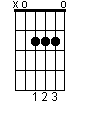
\includegraphics{partthree/openamajor.png}

This chord is a little tougher; you've got to fit all three of your fingers on the second fret, and it can feel a little crowded at first. Start by placing your first finger on the second fret of the fourth string. Next, put your second finger on the second fret on the third string. Lastly, place your third finger on the second fret of the second string. Strum the bottom five strings (being careful to avoid the sixth), and you'll be playing an Amajor chord.

Another common way to play an Amajor chord is by flattening one finger across the second fret of all three strings. This can be tricky, and initially, will be extremely difficult to play cleanly.

\section{Playing an F Major Chord}
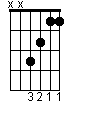
\includegraphics{partthree/openfmajor.png}

This chord has been left until last, because, honestly, it's a toughie. As the saying goes... "it's not called an F-chord for nothing!"

Many new guitarists have such a problem with the Fmajor chord because it involves a new concept; using your first finger to press down frets on two strings.

Start by placing your first finger on the first frets of both the first and second strings. Now, slightly roll the finger back (towards the headstock of the guitar). Many people find this technique makes playing the Fmajor chord slightly easier. Next, place your second finger on the second fret of the third string. Lastly, place your third finger on the third fret of the fourth string. Strum only the bottom four strings, and you're playing an Fmajor chord.

Chances are, at first, very few, if any of the notes will ring when trying to strum this chord. Check to make sure your second and third fingers are curled, and not flattened against the other strings of the guitar. Although this chord seems nearly impossible at first, within weeks, you'll have it sounding as good as the rest of the chords you play.

\section{Chord Review}
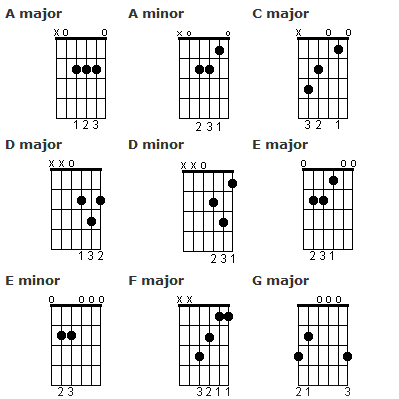
\includegraphics{partthree/lesson-three-chord-chart.png}

Including the three new chords in this week's lesson, we've now learned a total of nine chords. That might not seem like a whole lot, but at first, they can be hard to memorize. If you're having a hard time remembering all these chords, refer to the following archive.

\subsection{Practicing these chords}

Getting these chords memorized is just the first step. In order for them to be useful, you'll have to learn to move from chord to chord fairly quickly. This will take much practice and patience, but you'll get the hang of it!

Once you've reviewed these chords thoroughly, move on to learning a new strum. The main reason most beginners have trouble switching chords quickly is because of wasted movement in their fretting hand. Study your fingers when moving from chord to chord. Chances are, one (or a few) of your fingers will come way off the fretboard, and often hover in mid-air while you try to decide where each finger should go. This is unnecessary, and can really slow you down. Now, try again... play a chord, and BEFORE you switch to another chord, visualize playing this second chord shape. Picture in your mind exactly which fingers will need to go where, and only after you've done this should you switch chords. Pay attention to any small, unnecessary movements your fingers make, and eliminate them. Although this is easier said than done, your hard work and attention to detail will start paying off quickly.

\section{New Strumming Pattern}
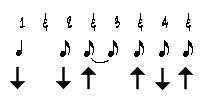
\includegraphics{partthree/strum3.jpg}

In lesson two, we learned all about the basics of strumming. If you still aren't comfortable with the concept and execution of basic guitar strumming, I suggest you return to that lesson and review.

This strum isn't much different from the one in lesson two. In fact, many guitarists find it slightly easier.

Before you try and play this pattern, take some time to learn what it sounds like. Listen to an mp3 clip of the strumming pattern, and try to tap along with it. Once you are comfortable with it, try it at a faster speed. Now pick up your guitar and try playing the pattern while holding down a Gmajor chord (be sure to use the exact upstrokes and downstrokes the diagram illustrates). If you're having trouble, put down the guitar and practice saying or tapping out the rhythm again, making sure to repeat it multiple times. If you don't have the correct rhythm in your head, you'll never be able to play it on guitar.

Remember to keep the up and down strumming motion in your picking hand constant - even when you're not actually strumming the chord. Try saying out loud "down, down up, up down up" (or "1, 2 and, and 4 and") as you're playing the pattern.

\subsection{Remember:}
\begin{itemize}
\item Make sure all strings are ringing clearly
\item Make sure the volume of your downstrums and upstrums are equal
\item Be careful not to strum too hard, as this can cause strings to rattle and produces an undesirable sound
\item Be careful not to strum too softly, as this will produce a "wimpy" sound. Your pick should be striking the strings with a firm, even stroke
\item Think of your elbow as being the top of a pendulum; your arm should swing up and down from it in a steady motion, never pausing at any time.
\item Having said that, the bulk of the picking motion should come from a rotation of the wrist, rather than from the forearm. Be sure not to keep your wrist stiff when playing.
\end{itemize}

\section{Learning Songs}
The addition of three new minor chords to this week's lesson gives us a total of nine chords to learn songs with. These nine chords will provide you with the opportunity to play literally hundreds of country, blues, rock, and pop songs. Give these songs a try:

House of the Rising Sun - performed by The Animals
NOTES: This song is a little tough at first; it uses five of the nine chords we've learned. Ignore the picking pattern for now - instead strum each chord six times quickly with only downstrums.
MP3: Amazon.com download

Last Kiss - performed by Pearl Jam
NOTES: this song is quite easy to play... it only uses four chords which repeat for the entire song. Use this week's strumming pattern for the song (play the pattern once for each chord).
MP3: Amazon.com download

Mr. Jones - performed by The Counting Crows
NOTES: This one might be tough, because it uses an Fmaj chord, and because some chords are held longer than others. Playing along with a recording of the song should help. Although this week's strumming pattern isn't exactly what they play, it will work fine.
MP3: Amazon.com download

American Pie - performed by Don McLean
NOTES: This one will be hard to memorize! It's very long, and has lots of chords, but it should be a good project. Ignore the 7ths... play Amin instead of Am7, Emin instead of Em7, and Dmaj instead of D7. Also, ignore the chords in the brackets for now.
MP3: Amazon.com download

\section{Practice Schedule}
I hope you're putting in your fifteen minutes of practice per day! It's not a lot of time to play guitar, but even fifteen minutes will yield good results over time. If you have the time to play more, it's highly encouraged... the more the better! Here's a suggested use of your practice time for the next few weeks.
\begin{itemize}
\item Make sure your guitar is in tune (review how to tune).
\item Warm up by playing the blues scale, forwards and backwards, several times. Play slowly, use alternate picking, and make sure each note rings clearly.
\item Play the E phrygian scale from lesson 2 several times, paying careful attention to detail.
\item Review all nine major and minor chords we've learned. Practice moving from chord to chord quickly.
\item Spend some time working on this week's new strumming pattern. Also, be sure to revisit the lesson two strumming patterns. Try switching from chord to chord while using these patterns.
\item Try to play one, or a few of the songs above. See if you can memorize part of a song, and the lyrics to the song. At this point, songs probably won't sound great when you try and play them, but with some patience, you'll be sounding like a pro within months! 
\end{itemize}
As was suggested in lesson two, if you find it impossible to find the time to practice all of the above in one sitting, try breaking up the material, and practicing it over several days. There is a strong human tendency to only practice things which we are already quite good at. You'll need to overcome this, and force yourself to practice the things you are weakest at doing.

